\section{Knowing How with Linear Plans}
\label{sec:khlinearplans}

\subsection{Basic Definitions}

We start by introducing the most basic notion of knowing how as defined in e.g.~\cite{Wang15lori,Wang16,Wang2016}.


\begin{definition}\label{def:lts}
    Let $\PROP$ be a countable set of propositional symbols. 
    A \emph{Labeled Transition System (LTS)}  is a tuple
    $\model=\tup{\S,\ACT,\ra,\V}$ such that:
    \begin{itemize}
        \item $\S$ is a countably non-empty set of states,
        \item $\ACT$ is a countable set of action symbols,
        \item ${\ra} \subseteq \S \times \ACT \times \S$ is a transition relation (sometimes we denote by $\reach{a}$ the set $\set{(s,t) \mid (s,a,t){\in}{\ra}}$, for $a\in\ACT$).
    \end{itemize}
    Elements of $\ACT^*$ are called \emph{plans} (with $\epsilon$ the empty plan).  Let $\plan\in\ACT^*$, $\size{\plan}$ denotes its length ($\size{\epsilon}:=0$).
    For  $0\leq i \leq \size{\plan}$, the plan $\plan_i$ denotes the initial segment of $\plan$ up to (and including) the $i^{th}$ position (with $\plan_0 := \epsilon$). The action $\plan[i]$ is the one appearing in $\plan$ at the $i^{th}$ position. We define $\reach{\plan}$ as the composition $\reach{\plan[1]} \comp \ldots \comp \reach{\plan[\size{\plan}]}$. 

    We say that a plan $\plan\in\ACT^*$ is \emph{strongly executable (SE)} at a state $s\in\S$ if and only if, for all $0\leq i \leq \size{\plan}-1$ and all $t\in\S$ such that $s\reach{\plan_i} t$, there is $v\in\S$ such that $t\reach{\plan[i+1]} v$. The plan $\plan$ is SE at $T\subseteq \S$ if and only if it is SE at every $s\in T$.
\end{definition}

\begin{definition}
    \label{def:syntax}
    The set of formulas (a.k.a. the language) of $\Khlogic$ is defined by the following BNF:
    \[
        \varphi, \psi ::= p \mid \neg \varphi \mid \varphi \vee \psi \mid \kh(\psi,\varphi),
    \]
    where $p\in\PROP$. Other Boolean operators are defined as usual. Formulas of the form $\kh(\psi,\varphi)$ are read as \emph{``the agent knows how to achieve $\varphi$ given $\psi$''}
\end{definition}

\begin{definition} \label{def:semantics-kh}
    Let $\model = \tup{\S,\ACT,\ra,\V}$ be an LTS and let $s\in\S$, the satisfiability relation $\models$ for $\Khlogic$ is inductively defined as:
    \[
    \begin{array}{l@{\ \ \ }c@{\ \ \  }l}
    \model, s \models p & \iffdef & p \in \V(s) \\
    \model, s\models \neg\varphi & \iffdef & \model, s \not\models \varphi \\
    \model, s \models \psi\vee\varphi & \iffdef & \model, s \models \psi \mbox{ or }\model, w \models \varphi \\
    \model, s \models \kh(\psi,\varphi) & \iffdef & \text{there is } \plan \in \ACT^* \;\text{such that:} \\
    & & \ \ \text{\rm (1)} \ \plan \text{ is SE-executable at }  \truthset{\model}{\psi}\; \text{and} \\
    & & \ \ \text{\em (2)} \ \truthset{\model}{\psi} \reach{\plan} \truthset{\model}{\varphi}, 
    \end{array}
    \]      where: $\truthset{\model}{\chi} := \csetsc{s\in\S}{\model,w\models\chi}$. Define: $\model\models\varphi$ iff  $\truthset{\model}{\varphi}=\S$, and $\models\varphi$ iff $\model\models\varphi$, for all LTS $\model$.
\end{definition}

\subsection{The Probabilistic Approach}

\begin{definition}\label{def:plts}
    Let $\PROP$ be a countable set of propositional symbols. 
    A \emph{Probabilistic Labeled Transition System (PLTS)}  is a tuple
    $\model=\tup{\S,\ACT,\ra,\V}$, defined exactly as an LTS except that ${\ra}\subseteq \S \times \ACT \times \dist(\S)$, where  $\dist(\S)$ is the set of probability distributions over $\S$.
\end{definition}

    \begin{figure}[t]
        \begin{center}
            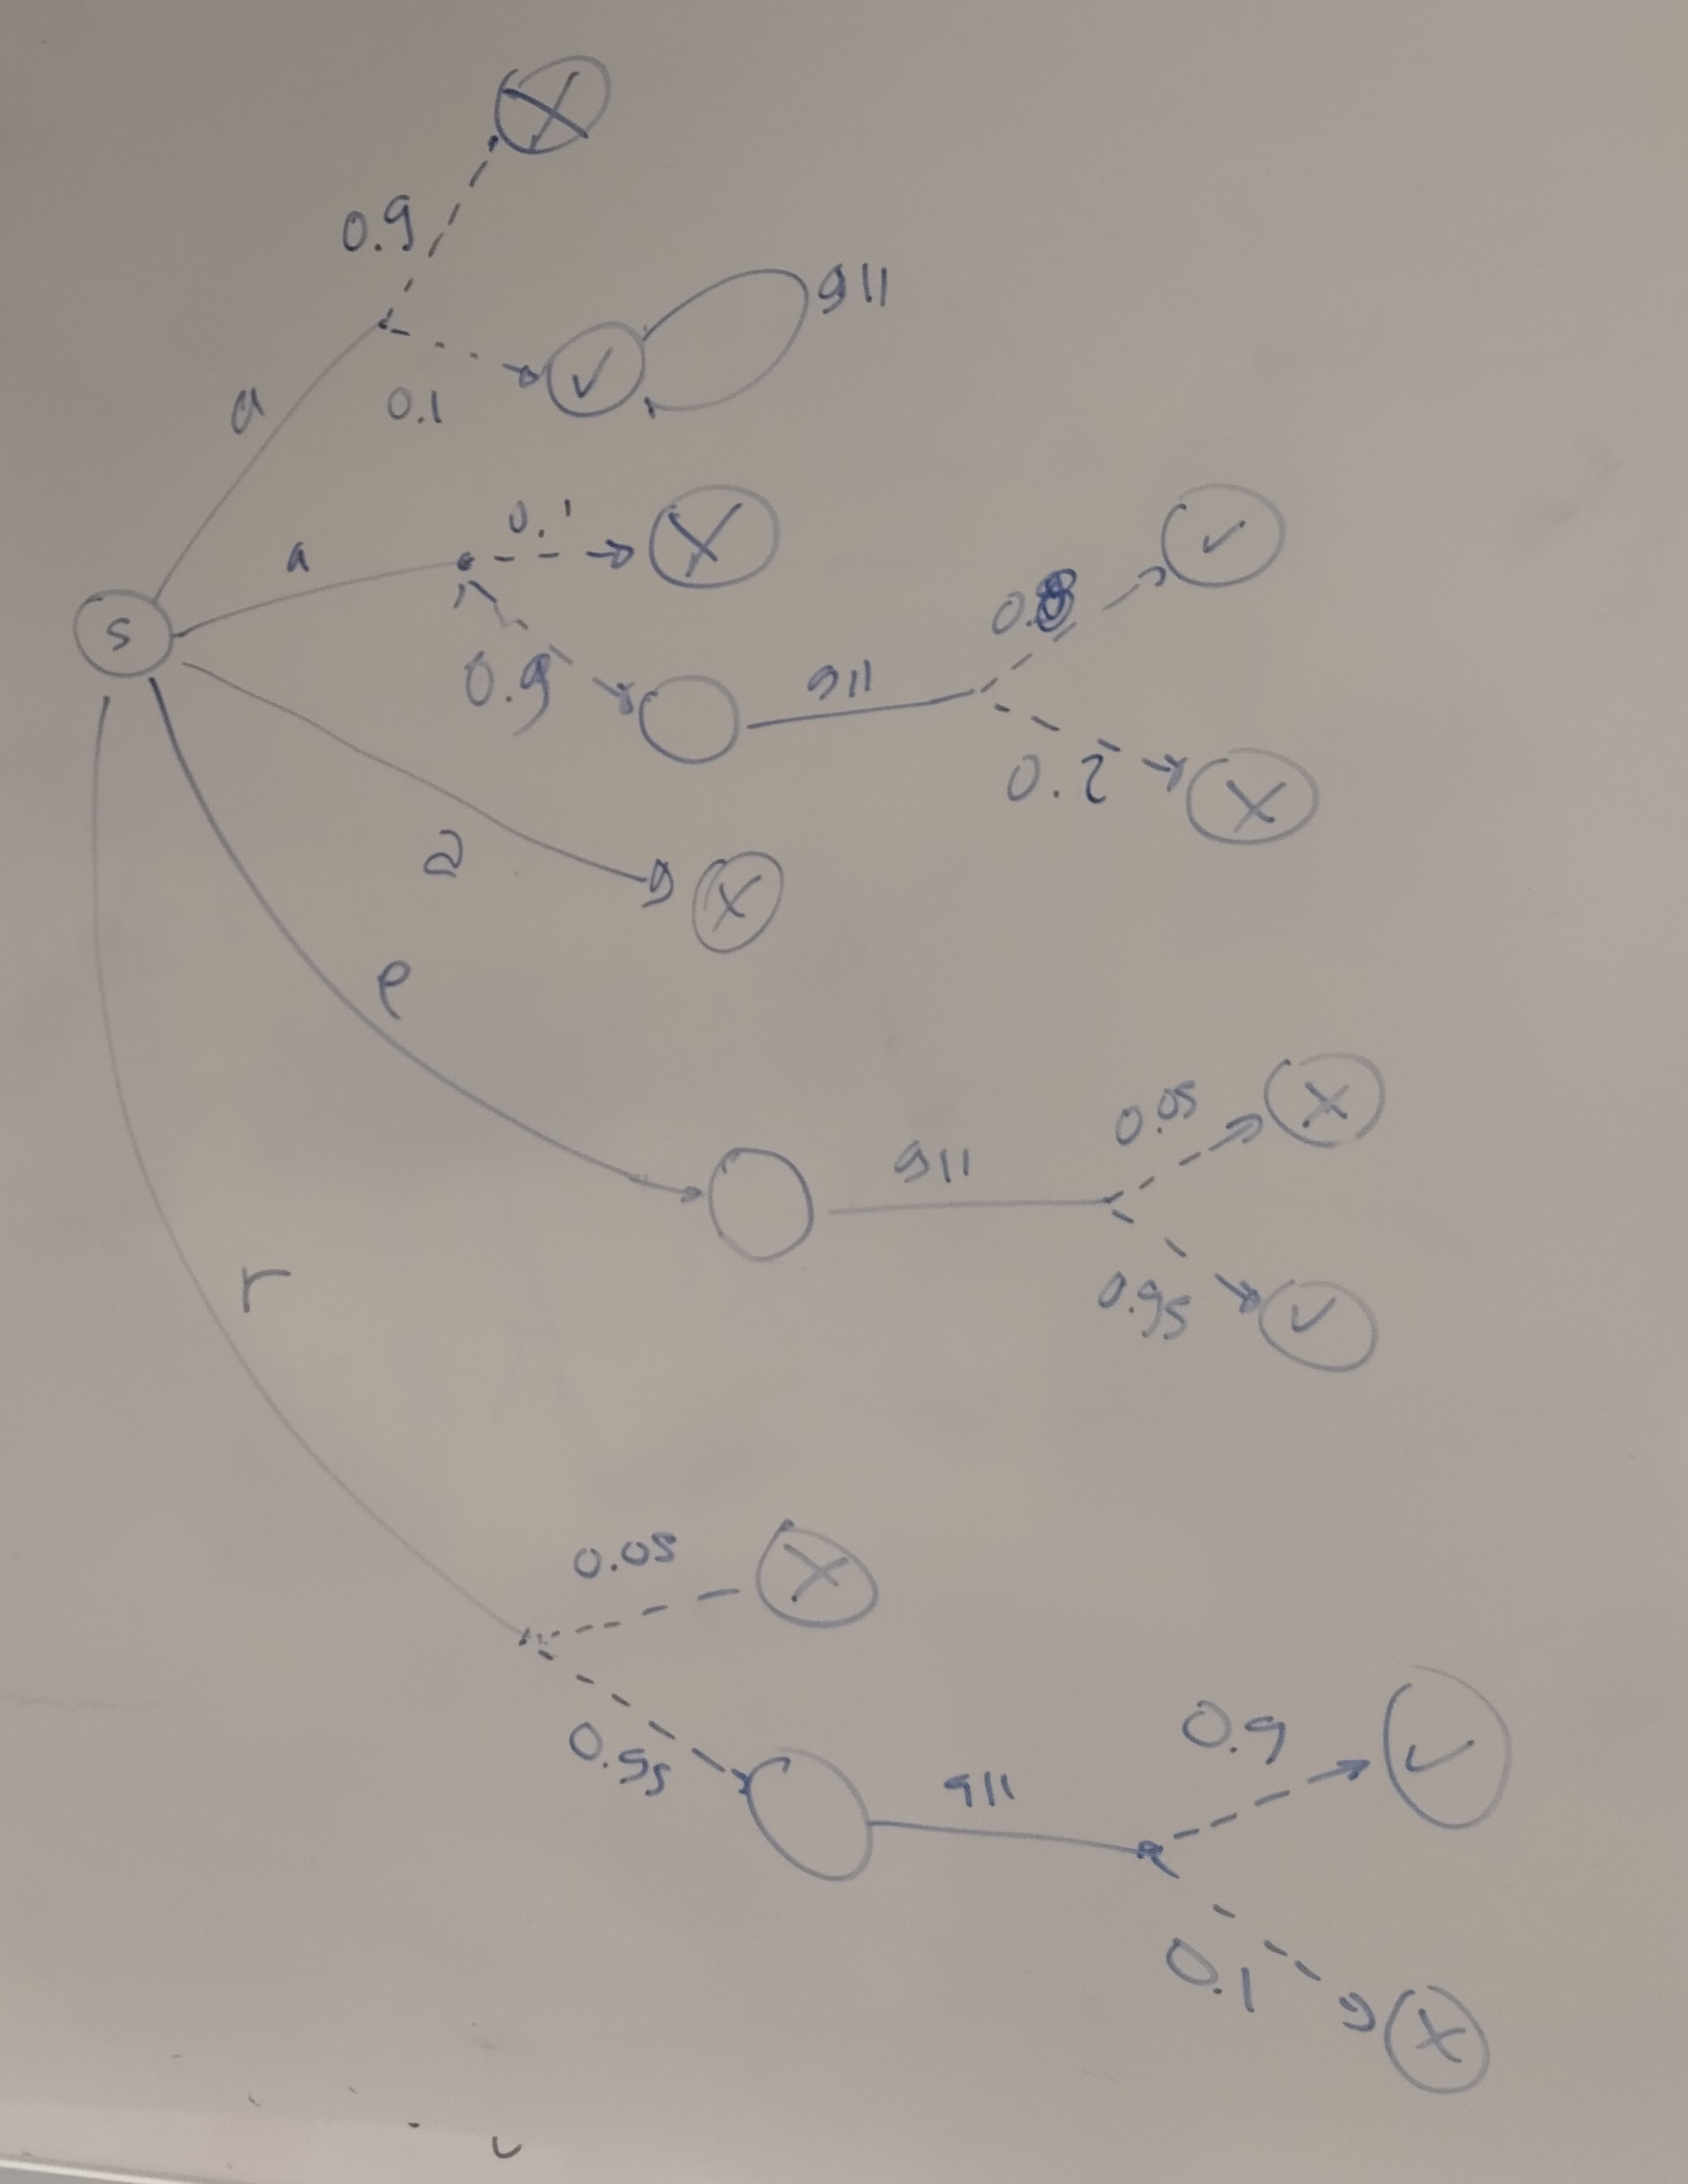
\includegraphics[scale=0.1]{PLTS.jpg}
        \end{center}
    \end{figure}

\begin{definition}\label{def:strategy-comp-exec}
    Let $\model=\tup{\S,\ACT,\ra,\V}$ be a PLTS, a \emph{strategy} is a function $\strategy: \S\times(\ACT\times\S)^* \ra \dist(\S\times\ACT\times\dist(\S))$. Let $\plan\in\ACT^*$, we say that $\strategy$ is \emph{$\plans$-compatible} if and only if, for all $\rho\in \S\times(\ACT\times\S)^*$, the following conditions hold:
    \begin{enumerate}
        \item $\strategy(\rho)(s,a,\mu)>0$ implies $\last(\rho)=s$ and $s\reach{a}\mu$ in $\model$, and 
        \item $\bar{\rho}\in\pref(\plans)$ implies $\bar{\rho}a\in\pref(\plans)$.
    \end{enumerate}
    For $\plan\in\ACT^*$, we say that $\sigma$ is \emph{$\plan$-compatible} if it is $\{\plan\}$-compatible. 

    Let $q\in[0,1]$, we say that $\plans$ is \emph{$q$-executable} at $s\in\S$, if and only if, 
    \[
        \infim_{\{\strategy \mid \strategy \text{ is } \plans\text{-comp.}\}} \probability^\strategy_{s}(\plans)\geq q.
    \]
    Finally, $\plans$ is \emph{$q$-executable} at $B\subseteq\S$, if and only if, it is $q$-executable at every $s\in B$. 
    A plan $\plan$ is \emph{$q$-executable} at $s$ (respectively, at $B$) if $\{\plan\}$ is $q$-executable at $s$ (respectively, at $B$). 
\end{definition}

\begin{definition}
    Let $\model = \tup{\S,\ACT,\ra,\V}$ be a PLTS and let $s\in\S$, the satisfiability relation $\models$ for $\PKh$ is inductively defined as:
    \[
        \begin{array}{l@{\ \ \ }c@{\ \ \  }l}
        % \model, s \models p & \iffdef & p \in \V(s) \\
        % \model, s\models \neg\varphi & \iffdef & \model, s \not\models \varphi \\
        % \model, s \models \psi\vee\varphi & \iffdef & \model, s \models \psi \mbox{ or }\model, w \models \varphi \\
        \model, s \models \kh^q(\psi,\varphi) & \iffdef & \text{there is } \plan \in \ACT^* \;\text{such that:} \\
        & & \ \ \text{\rm (1)} \ \plan \text{ is $q$-executable at }  \truthset{\model}{\psi}\; \text{and} \\
        & & \ \ \text{\em (2)} \ \truthset{\model}{\psi} \reach{\plan}_q \truthset{\model}{\varphi}, 
        \end{array}
        \] \raul{1 and 2 will be merged into one condition.}
        where: $\truthset{\model}{\chi} := \csetsc{s\in\S}{\model,w\models\chi}$. Define: $\model\models\varphi$ iff  $\truthset{\model}{\varphi}=\S$, and $\models\varphi$ iff $\model\models\varphi$, for all PLTS $\model$.
\end{definition}

\begin{theorem}\label{th:mc-khp-undecidable}
The model-checking problem for $\PKh$ is undecidable.
\end{theorem}

\begin{proof}
    Suppose we want to check whether $\model,s\models\kh^q(\psi,\varphi)$.  W.l.o.g., consider $\model$ is complete and deterministic. 
    From the semantics, we need to check if there is $\plan\in\ACT^*$ satisfying conditions (1) and (2). Consider condition (1), i.e., we need to check whether $\plan$ is $q$-executable at all $s\in\truthset{\model}{\psi}$. Fix such an $s$. Since $\model$ is deterministic and complete, it all boils down to check whether there is $\plan\in\ACT^*$ such that $\probability^\strategy_s(\plan)\geq q$ (notice that $\strategy$ is unique by determinism of $\model$). 
    The latter solves the problem of checking whether the language recognized by a probabilistic (deterministic) automata is empty, which is undecidable~\cite{MadaniHC99}. 
\end{proof}